\scanpage{14}
\figure{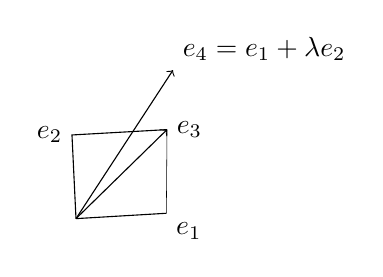
\begin{tikzpicture}[scale=.85]
\draw (0,0)--(1.35,.08) node[below right]{$e_1$};
\draw (0,0)--(-.06,1.25) node[left]{$e_2$}--(1.36,1.33) node[right]{$e_3$};
\draw[very thin] (1.35,.08)--(1.36,1.33);
\draw[->] (0,0)--(1.36,1.33);\draw[->] (0,0)--(1.45,2.22) node[above right]{$e_4=e_1+\lambda e_2$};
\end{tikzpicture}}

\[
\begin{aligned}e_3&=\begin{pmatrix}1\\1\end{pmatrix}\\e_4&=\begin{pmatrix}1\\\lambda\end{pmatrix}\end{aligned}
\]

\[
\boxed{\deleted{\unsure{\xi}}u=\begin{pmatrix}\unsure{\zeta|\xi}&0\\0&-\zeta\end{pmatrix}}
\qquad\begin{aligned}\operatorname{Tr}u&=0&\det u&=-\zeta^2\\\operatorname{Tr}v&=0&\det v&=-\eta^2\end{aligned}
\]

\[
\begin{aligned}
&\deleted{v=\bigl(\unsure{\eta}}\\
&v=\begin{pmatrix}a&b\\c&d\end{pmatrix}\deleted{\bigl(\unsure{0}}\qquad\deleted{v(e_1)=ae_1+ce_2}\\[-2pt]
&&\deleted{v(\unsure{.}}
\end{aligned}
\]

\[
\begin{aligned}
v(e_3)&=(a+b,c+d)=(\eta,\eta)\\
v(e_4)&=(a+\lambda b,c+\lambda d)=(-\eta,-\lambda\eta)
\end{aligned}
\qquad
\begin{aligned}a+b&=\eta\\c+d&=\eta\\a+\lambda b&=-\eta\\c+\lambda d&=-\lambda\eta\end{aligned}
\]

\[
\deleted{v=\begin{pmatrix}a&c\\c&a\end{pmatrix}}\qquad
\begin{aligned}b&=\eta-a\\d&=\eta-c\end{aligned}
\]

\[
\boxed{v=\begin{pmatrix}a&b\\-\lambda b&-a\end{pmatrix}}
\quad\left\{\begin{aligned}a&=\frac{\lambda+1}{\lambda-1}\eta\\
b&=\frac{-2}{\lambda-1}\eta\end{aligned}\right.
\]

\[
\begin{aligned}
a+\lambda(\eta-a)&=-\eta &(1-\lambda)\unsure{(|{}}a&=-(1+\lambda)\eta\\
c+\lambda(\eta-c)&=-\lambda\eta &(1-\lambda)c&=-2\lambda\eta
\end{aligned}
\]

\[
\begin{aligned}
\det v&=-a^2+\lambda \deleted{\unsure{4}}b^2=-\eta^2
\left[\underbrace{\left(\frac{\lambda+1}{\lambda-1}\right)^2-\lambda\frac{4}{(\lambda-1)^2}}_{\displaystyle\frac{(\lambda+1)^2-4\lambda}{(\lambda-1)^2}=1}\right]\\
&=
\end{aligned}
\]

\[
\begin{aligned}
a&=\frac{\lambda+1}{\lambda-1}\eta &b&=\unsure{.}\\
c&=\frac{+2\lambda\eta}{\lambda-1}\\
b&=\eta\left(1-\frac{\lambda+1}{\lambda-1}\right)=\frac{-2\deleted{\unsure{\lambda}}\eta}{\lambda-1}\deleted{\unsure{\eta}}\\
d&=\eta\left(1-\frac{\deleted{\unsure{4}}2\lambda}{\lambda-1}\right)=-\frac{\lambda+1}{\lambda-1}\eta=\deleted{\unsure{a}}\unsure{-|{}}a
\end{aligned}
\]

\[
\begin{aligned}
&\deleted{uv+vu}\\
uv&=\begin{pmatrix}\zeta a&\zeta b\\\deleted{\unsure{a}}\lambda\zeta b&\zeta a\end{pmatrix}
\qquad c=-\lambda b\\
vu&=\begin{pmatrix}\zeta a&-\zeta b\\-\lambda\zeta b&\zeta a\end{pmatrix}
\end{aligned}
\]

\[
uv+vu=\begin{pmatrix}2\zeta a&0\\0&2\zeta a\end{pmatrix}
=\deleted{\unsure{2\zeta\eta\frac{\lambda+1}{\lambda-1}.1|2\zeta a\frac{\lambda+1}{\lambda-1}.1}}\;2\zeta a.1
\qquad 2\zeta a=\operatorname{Tr}vu
\]

% archive sheet number: 13
